\scanpage{33}
\mspage{14}
\figure{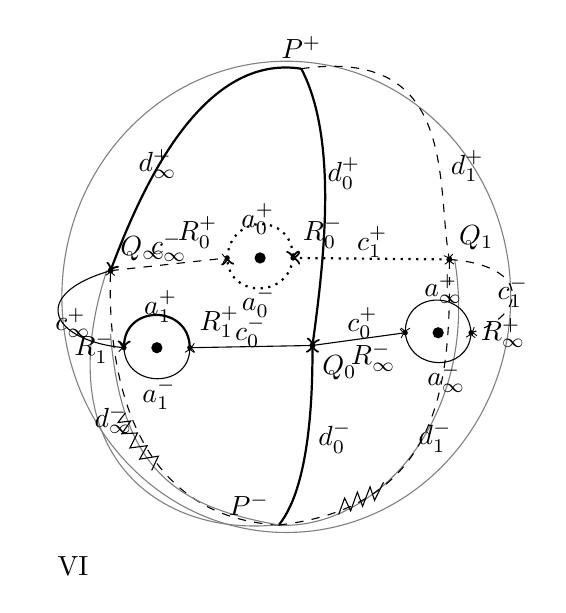
\begin{tikzpicture}[scale=.95]
\draw[gray] (0,0) ellipse (3 and 3.15);
\draw[gray] (-2.4,.35)..controls (-3.2,-2.1) and (-1.7,-3.2)..(-.15,-3.05);
\draw[gray] (2.25,.5)..controls (2.6,-1.6) and (1.2,-3.15)..(-.15,-3.05);
\coordinate (Pp) at (.2,3.05);\coordinate (Pm) at (-.1,-3.05);
\coordinate (Qi) at (-2.35,.35);\coordinate (Qz) at (.35,-.65);\coordinate (Qo) at (2.18,.5);
\draw[->,thick] (Pp)..controls (-1.1,3.25) and (-1.9,1.55)..(Qi);
\draw[->,thick] (Pp)..controls (.7,2.1) and (.5,.45)..(Qz);
\draw[dashed,->] (Pp)..controls (2.3,3.35) and (2,1.5)..(Qo);
\draw[dashed,->] (Pm)..controls (-1.95,-2.95) and (-2.4,-1.2)..(Qi);
\draw[->,thick] (Pm)..controls (.35,-2.5) and (.35,-1.1)..(Qz);
\draw[dashed,->] (Pm)..controls (2.1,-2.8) and (2.2,-1.1)..(Qo);
\draw[gray] (-2.35,-.5)..controls (-2.2,-2.3) and (-1.5,-2.8)..(-.1,-3.05);
\draw (-2.15,-1.55)--(-2.25,-1.68)--(-2.08,-1.66)--(-2.2,-1.83)--(-1.99,-1.82)--(-2.09,-2.02)--(-1.86,-1.99)--(-1.96,-2.17)--(-1.71,-2.13)--(-1.8,-2.32);
\draw (.7,-2.91)--(.78,-2.69)--(.86,-2.86)--(.95,-2.61)--(1.02,-2.8)--(1.12,-2.54)--(1.18,-2.72)--(1.3,-2.48);
\foreach \p in {Qi,Qz,Qo}{\fill (\p) circle (.04);}
\node[above] at (Pp) {$P^+$};\node[above left] at (Pm) {$P^-$};
\node[above right] at (Qi) {$Q_\infty$};\node[below right] at (Qz) {$Q_0$};\node[above right] at (Qo) {$Q_1$};
\node at (-1.72,1.78) {$d_\infty^+$};\node at (.77,1.65) {$d_0^+$};\node at (2.42,1.75) {$d_1^+$};
\node at (-2.31,-1.64) {$d_\infty^-$};\node at (.65,-1.88) {$d_0^-$};\node at (1.99,-1.87) {$d_1^-$};
\fill (-.35,.52) circle (.075);\fill (-1.73,-.68) circle (.075);\fill (2.03,-.48) circle (.075);
\coordinate (Rzp) at (-.79,.52);\coordinate (Rzm) at (.09,.52);
\coordinate (Rom) at (-2.17,-.68);\coordinate (Rop) at (-1.29,-.68);
\coordinate (Rim) at (1.59,-.48);\coordinate (Rip) at (2.47,-.48);
\draw[dotted,thick,->] (Rzp)..controls (-.75,1.12) and (.07,1.12)..(Rzm);
\draw[dotted,thick,->] (Rzm)..controls (.03,-.02) and (-.75,-.02)..(Rzp);
\draw[->,thick] (Rop)..controls (-1.3,-.1) and (-2.16,-.1)..(Rom);
\draw[->] (Rom)..controls (-2.15,-1.23) and (-1.3,-1.23)..(Rop);
\draw[->] (Rip)..controls (2.43,.1) and (1.6,.1)..(Rim);
\draw[->] (Rim)..controls (1.65,-1.01) and (2.43,-1.01)..(Rip);
\foreach \p in {Rzp,Rzm,Rom,Rop,Rim,Rip}{\fill (\p) circle (.035);}
\node[above left] at (Rzp) {$R_0^+$};\node[above right] at (Rzm) {$R_0^-$};
\node[left] at (Rom) {$R_1^-$};\node[above right] at (Rop) {$R_1^+$};
\node[below left] at (Rim) {$R_\infty^-$};\node[right] at (Rip) {$R_\infty^+$};
\node at (-.38,1.04) {$a_0^+$};\node at (-.37,-.07) {$a_0^-$};
\node at (-1.68,-.13) {$a_1^+$};\node at (-1.7,-1.3) {$a_1^-$};
\node at (2.1,.11) {$a_\infty^+$};\node at (2.14,-1.08) {$a_\infty^-$};
\draw[dashed,->] (Qi)--(Rzp);\node at (-1.57,.67) {$c_\infty^-$};
\draw[->] (Qi)..controls (-3.45,.03) and (-3.15,-.58)..(Rom);\node at (-2.85,-.35) {$c_\infty^+$};
\draw[dotted,thick,->] (Qo)--(Rzm);\node at (1.15,.73) {$c_1^+$};
\draw[dashed,->] (Qo)..controls (3.3,.42) and (3.2,-.26)..(Rip);\node at (3.03,.07) {$c_1^-$};
\draw[->] (Qz)--(Rop);\node at (-.48,-.47) {$c_0^-$};
\draw[->] (Qz)--(Rim);\node at (1.02,-.35) {$c_0^+$};
\node at (-2.85,-3.6) {$\mathrm{VI}$};
\end{tikzpicture}}
C'est le groupoïde engendré par ces sommets, les arêtes $a_i^\omega,c_i^\omega,d_i^\omega$ (trois paquets, \deleted{\unsure{permutés}} \inserted{ch. un} un torseur sous $G_J$) et les \inserted{\unsure{six}} relations
\[
(48)\qquad(d_{\omega i}^\omega)^{-1}(c_{\omega i}^{\omega'})^{-1}(a_{\omega i}^\omega)^{-1}c_i^\omega d_i^\omega=1
\]
\deleted{\unsure{Hom.}} L'automorphisme $\tau$ est donné par
\[
(49)\qquad\left\{\begin{aligned}
\tau(R_i^\omega)&=R_i^{\unsure{\omega|\omega'}},&\tau Q_i&=Q_i,&\tau(P_{\deleted{\unsure{\infty}}}^\omega)&=P^{\omega'}\\
\tau(a_i^\omega)&=(a_i^{\omega'})^{-1},&\tau(c_i^\omega)&=c_i^{\unsure{\omega'|\omega}},&\tau(d_i^\omega)&=d_i^{\omega'}
\end{aligned}\right.
\]
Les $\pi_1\unsure{\varepsilon}$ de les sommets $R_i^\omega,Q_i,P^\omega$ sont repérés respectivement, en termes de $\Pi_{0,3}$, par \unsure{ces|les} isomorphismes
\[
(50)\qquad\left\{\begin{gathered}
\begin{tikzcd}[ampersand replacement=\&,column sep=large]
\Pi_{0,3}\arrow[r,"\varphi_i^\omega"]\&\pi(R_i^\omega)\deleted{\longrightarrow\pi(}
\end{tikzcd}\\
\begin{tikzcd}[ampersand replacement=\&,column sep=large]
\Pi_{0,3}\arrow[r,"\psi_i^\omega"]\&\pi(Q_i)
\end{tikzcd}\\
\begin{tikzcd}[ampersand replacement=\&,column sep=large]
\Pi_{0,3}\arrow[r,"\widetilde\psi_i^\omega"]\&\pi(P^\omega)
\end{tikzcd}
\end{gathered}\right.
\]
reliés entre eux par les relations suivantes, qui \deleted{les} expriment \deleted{les} \inserted{les $\psi_i^\omega,\widetilde\psi_i^\omega$} en termes des $\varphi_i^\omega$
\[
(51)\qquad\deleted{\unsure{\widetilde d_i^\omega}}\left\{\begin{aligned}
d_i^\omega(\widetilde\psi_i^\omega(g))&=\psi_i^\omega(g)\\
\deleted{\unsure{\psi_i^\omega}}c_i^\omega\psi_i^\omega(g)&=\varphi_i^\omega(g)
\end{aligned}\right.
\]
On a, pour mémoire
\[
(52)\qquad\psi_i^\omega(g)=\psi_i^{\omega'}(\sigma_\infty(g))
\]
\margin{32}
